\subsection{Generierung von Dateien}\label{subsec:generierung-von-dateien}
Aus einer Workflow-Beschreibung können bis zu fünf verschiedene Typen von Dateien generiert werden.
Der Einstiegspunkt und somit der Start des Parsens und der Generierung ist die \textit{BoardGenerator}-Klasse.
Diese hat Methoden, um Datei- oder String-Eingaben zu verarbeiten.
Nachdem mittels des Parsers aus der Eingabe ein fertiges Board-Objekt erstellt wurde, werden weitere Klassen zur Generierung verwendet.
HTML-Dateien werden vom HtmlGenerator generiert, hierbei handelt es sich um Mockups und das \ac{ES}-Board.
Mockups können allerdings auch als FXML-Datei generiert werden, um eine Grundlage für eine JavaFx-Anwendung zu bilden.
Diese Generierung übernimmt der FxmlGenerator.
Zuletzt vereint der DiagramGenerator die Generierung von Objekt- und Klassendiagrammen.
Außer der \textit{BoardGenerator}-Klasse sind die restlichen Generator-Klassen für die Vorbereitung der Daten zuständig.
Diese erhalten Eingaben von dem BoardGenerator, bereiten diese Eingabe auf, je nachdem welche Daten benötigt werden und enthalten eine
separate Methode zum Erstellen von Dateien im Dateisystem.
Das Bauen einer Datei in Form eines Strings wird in einer gesonderten \textit{Constructor}-Klasse erledigt.
Da es fünf verschiedene Typen von Dateien gibt und das Bauen für jede Datei unterschiedlich ist, existiert für jeden Typ eine eigene~\textit{Constructor}-Klasse.
Im Folgenden werden die Aufbereitungsschritte genauer beleuchtet.

\subsubsection{Event-Storming-Board}
Für die Generierung des Event-Storming-Boards bedarf es keiner Bearbeitung des HtmlGenerators, da das gesamte Board generiert werden soll und die Daten,
welche vom Parser erstellt wurden, bereits optimiert sind.
Die HTML-Datei wird mittels~\acp{ST}, welche in einer~\ac{STG} organisiert sind, zusammengebaut.
Für jeden Workflow im Board-Objekt wird eine neue Reihe in der HTML-Datei angelegt.
Innerhalb einer Workflow-Reihe werden alle dazugehörigen Notes gebaut.
Hierbei wird zwischen den verschiedenen Notes unterschieden, um verschiedene Darstellungen zu ermöglichen.
Je nach Note wird eines von drei ~\acp{ST} verwendet.
Für die Standard-Notes wird eine neue~\textit{Card}, eine Bootstrap-CSS-Klasse, erstellt, welche den Typen des Notes, dessen Content und eine bestimmte Farbe übergeben bekommt.
Für die organisatorischen Notes, User, Service und ExternalSystem, wird eine Card erstellt, welche kleiner als die eines normalen Notes ist.
Zudem wird in organisatorischen Notes nur ein Icon und der Bezeichner angezeigt, wobei das Icon ein Bootstrap-Icon ist.
Data- und Page-Notes werden gesondert mit einem dritten ~\ac{ST} behandelt, da es neben Typ, Content und Farbe noch einen Link gibt, welcher als Button definiert und für die Verwendung
im Web-Editor genutzt wird.

\begin{figure}[h]
    \centering
    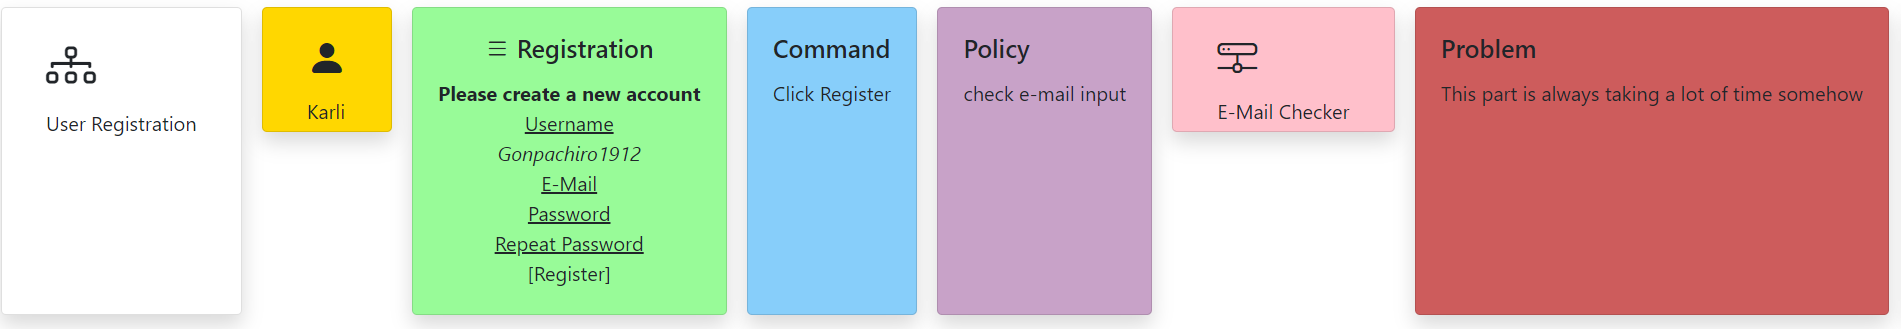
\includegraphics[width=1.0\textwidth]{images/3.1.4/board}
    \caption{Mittels fulibWorkflows generiertes Event-Storming-Board}
    \label{fig:generated-board}
\end{figure}

In Abbildung~\ref{fig:generated-board} ist ein Ausschnitt des in Listing~\ref{listing:workflowNotes} beschriebenen Workflows in
Form eines generierten \ac{ES}-Boards dargestellt.
Hierbei sind die zuvor beschriebenen Unterschiede zwischen den verschiedenen Notes erkennbar.
Jeder Note-Typ besitzt eine eigene Farbe, wobei für User, Service und ExternalSystem eine kleinere Card und jeweils ein
eigenes Icon erkennbar sind.
Der Page-Note enthält die meisten Informationen, da nur dort zusätzliche Informationen in der Workflow-Beschreibung existierten.

\subsubsection{Mockups (HTML und FXML)}\label{subsubsec:mockups-html/fxml}
Die Generierung von HTML-Mockups wird durch die~\textit{HtmlGenerator}-Klasse übernommen.
Diese filtert aus allen Workflows und den dazugehörigen Notes die Pages heraus und übergibt diese an die \textit{PageConstructor}-Klasse.
FXML-Mockups erhalten eine gesonderte Generator- und Constructor-Klasse.
Die in diesen Klassen befindlichen Funktionen ähneln der Funktionsweise des HtmlGenerators und PageConstructors stark.
Eine Unterscheidung in HTML und FXML wurde vorgenommen, um bei der Generierung die Möglichkeit von verschiedenen Optionen offenzulassen.
Somit könnten entweder nur HTML- oder FXML-Mockups erstellt werden.
Der FxmlConstructor und PageConstructor haben somit sowohl eine ähnliche Funktionsweise als auch einen ähnlichen Aufbau, da die zugrundeliegenden Daten gleich sind.
Lediglich die zugrunde liegende~\ac{STG} unterscheidet die beiden Klassen.
In beiden~\acp{STG} gibt es ein~\ac{ST} zum Aufbau der generellen Struktur der jeweiligen Datei und für jedes verfügbare Oberflächenelement ein weiteres~\ac{ST}.
Es existieren somit für die Oberflächenelemente~\acp{ST} für Text, Eingabefeld, Passwortfeld und Knopf.

\begin{figure}%
    \centering
    \subfloat[\centering FXML-Mockup]{{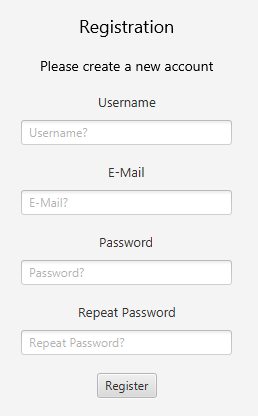
\includegraphics[width=4cm,height=6cm]{images/3.1.4/fxml-mockup} }}%
    \qquad
    \subfloat[\centering HTML-Mockup]{{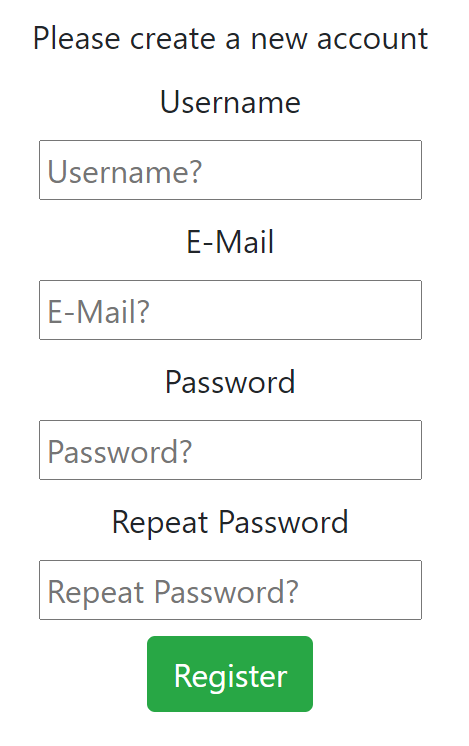
\includegraphics[width=4cm,height=6cm]{images/3.1.4/html-mockup} }}%
    \caption{Mittels fulibWorkflows generierte Mockups}%
    \label{fig:mockups}%
\end{figure}

In Abbildung~\ref{fig:mockups} sind die generierten Mockups aus dem vorherigen Beispiel dargestellt.
Diese bestehen, entsprechend der Beschreibung, aus einem Text, drei Eingabefeldern, einem Passwortfeld und einem Knopf.
Bei der Generierung wird vor allem darauf geachtet, dass sich die Oberflächen möglichst stark ähneln.
Der Aufbau der in Abbildung~\ref{fig:mockups}((a)) und Abbildung~\ref{fig:mockups}((b)) dargestellten Oberflächen ist somit grundlegend gleich.
Unterschiede entstehen einzig durch die verschiedenen Styles, da in dem HTML-Mockup Bootstrap zum Stylen der Oberfläche verwendet wurde.
Zudem ist erkennbar, dass das Username-Eingabefeld bei dem FXML-Mockup (links) leer ist, allerdings ist dieses mit den im Beispiel definierten
Daten im HTML-Mockup (rechts) bereits befüllt.
Diese Wahl wurde getroffen, da die beiden Mockup-Typen verschiedene Anwendungszwecke haben.
Die HTML-Mockups können im Web-Editor angezeigt werden und somit direkt mit den am Event Storming teilnehmenden Personen angeschaut werden.
Dies ist mit den FXML-Mockups nicht möglich, da diese ausschließlich zur Grundlage einer Benutzeroberfläche in einer Java-Anwendung werden.

\subsubsection{Objektdiagramme}\label{subsubsec:objektdiagramme}
Zuletzt gibt es die \textit{DiagramGenerator}-Klasse, welche die Eingabe für Objekt- und Klassendiagramme aufarbeitet.
Jeder Data-Note erhält sein eigenes Objektdiagramm.
Damit die zeitliche Abfolge und somit ein korrektes Objektdiagramm entsteht, wird jeder Data-Note zu einer Liste hinzugefügt und diese anschließend an die
\textit{ObjectDiagramConstructor}-Klasse übergeben.
Hierdurch werden pro Data-Note mehr Objekte zu dem dazugehörigen Objektdiagramm hinzugefügt, sollte es eine Verbindung zu einem bestehenden Objekt geben.
FulibTools verwendet Graphviz zur Erstellung von Diagrammen, zusätzlich gibt es die Möglichkeit Objekt- und Klassendiagramme anhand einer bestimmten Eingabe zu generieren.
Diese Funktionalität macht sich fulibWorkflows im ObjectDiagramConstructor zunutze.
Aus der übergebenen Liste an Data-Notes wird eine YAML-Datei erstellt, welche den Spezifikationen von fulibYaml entspricht.
In Listing~\ref{listing:fulibYaml} ist die zum ObjectDiagramConstructor gehörende \ac{STG}-Datei abgebildet.
Ein Objekt benötigt immer einen Namen, eine Klasse, in Zeile 5 als \textit{type} gekennzeichnet, und optionale Attribute.
Die Form eines Attributes ist in dem \ac{ST} ab Zeile 10 abgebildet, ein Attribute besteht lediglich aus einer Klasse, erneut \textit{type} genannt, und dem
dazugehörigen Wert.

\begin{listing}[!ht]
    \inputminted{c}{listings/3.1.4/FulibYaml.stg}
    \caption{FulibYaml.stg}
    \label{listing:fulibYaml}
\end{listing}

Nachdem ein Objektdiagramm in fulibYaml-Notation vorhanden ist, wird FulibTools verwendet, um daraus ein Diagram zu generieren.
In Listing~\ref{listing:object-gen} ist diese Generierungsmethode abgebildet.
Der erste Parameter der Methode enthält die Objektstruktur in Form von fulibYaml als String.
Daraus wird in Zeile 99 und 100 ein root-Objekt erstellt, welches die Klasse \textit{YamlIdMap} aus der Bibliothek fulibYaml nutzt.
Dieses root-Objekt wird gemeinsam mit dem in Zeile 96 festgelegten Dateinamen durch FulibTools in Zeile 102 generiert.
FulibTools erlaubt bei der Generierung nicht, dass der Inhalt der zu generierenden Datei zurückgegeben wird, die Datei wird sofort im Dateisystem erstellt.

\begin{listing}[!ht]
    \inputminted[firstnumber=95]{java}{listings/3.1.4/ObjectGeneration.java}
    \caption{Generierungsmethode eines Objektdiagramms}
    \label{listing:object-gen}
\end{listing}

Im Anschluss an die Generierung durch FulibTools wird der Inhalt der generierten Datei als String ausgelesen und von der Methode zurückgegeben.
Danach wird die generierte Datei, sowie ein für die Generierung temporär angelegter Ordner wieder gelöscht.
Dies hat den Hintergrund, dass die Generierung von Dateien, in Form vom Speichern im lokalen Dateisystem, gesammelt in der BoardGenerator-Klasse vollzogen werden soll.
Zudem wird im BoardGenerator die Möglichkeit geboten, Dateien aus einer Workflow-Beschreibung zu generieren und diese als String zurückzugeben.
Diese Methoden existieren für die Nutzung im fulibWorkflows-Web-Editor, welche in einem nachfolgenden Kapitel näher betrachtet werden.

\begin{figure}%
    \centering
    \subfloat[\centering Diagramm nach 3 Data-Notes]{{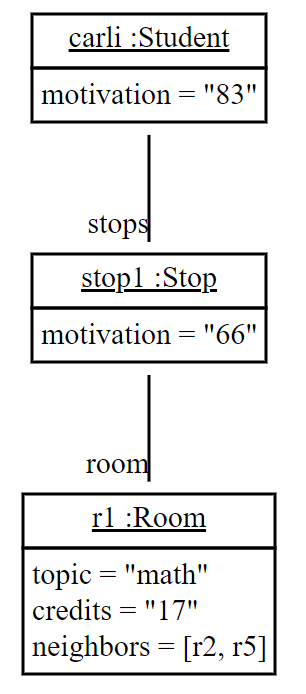
\includegraphics[width=2.5cm,height=6cm]{images/3.1.4/3_diagram} }}%
    \qquad
    \subfloat[\centering Diagramm nach 5 Data-Notes]{{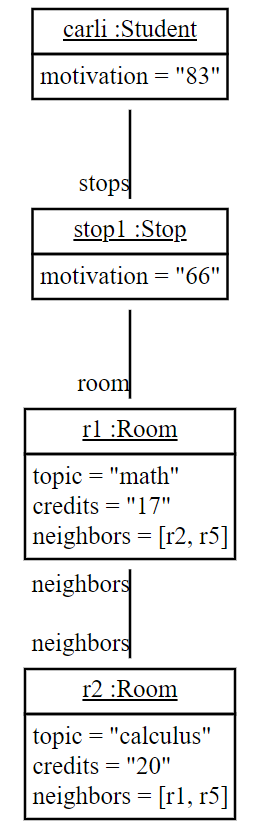
\includegraphics[width=2.5cm,height=7cm]{images/3.1.4/5_diagram} }}%
    \caption{Mittels fulibWorkflows generierte Objektdiagramme}%
    \label{fig:generated-object}%
\end{figure}

In Abbildung~\ref{fig:generated-object} sind zwei Objektdiagramme dargestellt, welche mit fulibWorkflows generiert wurden.
Die Beschreibung des Workflows stammt von einem Beispiel, welches zum Testen dieser Funktionalität in fulibWorkflows verwendet wurde.
Das Beispiel ist im Anhang in Listing~\ref{listing:pm-yaml} hinterlegt.
Zu dem Objektdiagramm aus Abbildung~\ref{fig:generated-object}((a)) ist ein weiteres Room-Objekt in Abbildung~\ref{fig:generated-object}((b)) hinzugefügt worden.
Dies basiert auf der vorher erwähnten Funktion, dass Objekte in einer Liste gespeichert werden und jedes neue Objekt dort hinzugefügt wird, bevor ein Objektdiagramm generiert wird.

\subsubsection{Klassendiagramme}
Der im vorherigen Kapitel eingeführte DiagramGenerator verwaltet nicht nur die Objektdiagramme.
Nachdem alle Data-Notes aus allen Workflows durchlaufen wurden, enthält der Generator eine Liste aller Data-Notes eines \ac{ES}-Boards.
Diese Liste wird an die \textit{ClassDiagramConstructor}-Klasse weitergegeben.

Für das Erstellen eines Klassenmodells müssen die Data-Notes bestimmte Spezifikationen erfüllen, um das gewünschte Ergebnis zu erzielen.

\begin{listing}[!ht]
    \inputminted[firstnumber=5]{yaml}{listings/3.1.4/data.es.yaml}
    \caption{Beispiel eines richtigen Data-Notes}
    \label{listing:object-yaml}
\end{listing}

Anhand des Data-Notes aus Listing~\ref{listing:object-yaml} werden folgend die eben erwähnten Spezifikationen näher betrachtet.
Der \textit{Name}, welcher in Zeile 5 nach dem Doppelpunkt vergeben wird, muss immer die Form: <Klassenname> <Objektname> besitzen.
Zudem muss beim ersten Aufkommen einer Assoziation sowohl die Hin- als auch Rückrichtung beschrieben werden.
Eine Assoziation wurde in Zeile 7 und 8 definiert, bei dieser wird mittels \textit{stops} der Bezeichner für die Hinrichtung festgelegt.
Mit den eckigen Klammern um dem Text \textit{stop1} wird ausgesagt, dass die Hinrichtung eine To-Many-Assoziation ist, somit ein Student mehrere Stops haben kann.
Damit die Verknüpfung von zwei Objekten funktioniert, benötigt es einen weiteren Data-Note, welcher ein Objekt ``stop1'' mit dem Typ ``Stop'' beschreibt.
Ein solcher zweiter Note ist in Zeile 10 dargestellt.
Die Rückrichtung wird in Zeile 8 durch \textit{stops.back} definiert, gemeinsam mit dem Wert \textit{student} wird der Bezeichner
der Rückrichtung auf \textit{student} gesetzt.
Durch die fehlenden eckigen Klammern ist die Kardinalität der Rückrichtung 0 oder 1.

\begin{listing}[!ht]
    \inputminted[firstnumber=39]{java}{listings/3.1.4/ClassProcedure.java}
    \caption{Schritte zum Aufbau eines Klassenmodells}
    \label{listing:class-procedure}
\end{listing}

Anhand dieser Anforderungen an einen Data-Note ist es möglich ein Klassenmodell aus den Notes zu abstrahieren.
In Listing~\ref{listing:class-procedure} sind die Schritte, welche zum Aufbau eines Klassenmodells nötig sind, aufgelistet.
Diese stammen samt Kommentaren aus der Implementierung der \textit{ClassModelManager}-Klasse in der fulib-Bibliothek.
Im ersten Schritt, Zeile 43, werden alle Klassen in einer Map abgelegt, wobei als Key der Name der Klasse und als Value ein \textit{Clazz}-Objekt fungiert.
Hierbei wird über alle Data-Notes iteriert und die darin enthaltenen Klassen aus dem Namen des Data-Notes extrahiert.
In Schritt zwei, Zeile 47, werden die vorhandenen Assoziationen erstellt.
Hierfür wurde eine Klasse namens \textit{Association} erstellt, welche zum Zwischenspeichern der für eine Assoziation wichtigen Daten speichert.
Darunter zählen Klasse, Bezeichner und Kardinalität für Hin- und Rückrichtung.
Neben diesen Daten werden in einer Liste von Strings Schlüsselwörter gespeichert, welche als Assoziation fungieren und nicht als Attribut betrachtet werden dürfen.
Die wichtigsten Spezifikationen für eine funktionierende Assoziation wurde bereits zuvor anhand von Listing~\ref{listing:object-yaml} erläutert.
Weiterhin ist es wichtig, dass die verwendeten Objektnamen in der Workflow-Beschreibung konsistent sind, da ansonsten keine Zielklasse ermittelt werden kann.
Während des Aufbaus einer Assoziation wird über alle Data-Notes iteriert, um die Informationen der Zielklasse zu erhalten.
Der nächste Schritt, Zeile 50, erstellt Attribute für alle Klassen.
Hierbei kommt die zuvor erstellte Liste an Schlüsselwörtern zum Tragen, um auszuschließen, dass eine Assoziation ebenfalls als Attribut aufgefasst wird.
Im letzten Schritt zur Abstrahierung eines Klassenmodells aus den Data-Notes werden die zuvor in Zeile 47 gebauten Assoziationen im Klassenmodell erstellt.
In diesem Schritt wird darauf geachtet, dass alle benötigten Informationen für eine Assoziation vorhanden sind.
Durch die Nutzung von fulib und dem ClassModelManager muss nicht auf Duplikate bei Attributen oder Assoziationen geachtet werden.

Nachdem das Klassenmodell erstellt wurde, wird dieses ebenfalls mit FulibTools zu einem Diagram weiterverarbeitet.
Der Ablauf hierbei ist ähnlich zu der Generierung von Objektdiagrammen.
Nachdem das Diagramm generiert wurde, wird dieses ebenfalls auf dem Dateisystem gelöscht und der Inhalt des Diagramms als String zurückgegeben.

\begin{figure}[h]
    \centering
    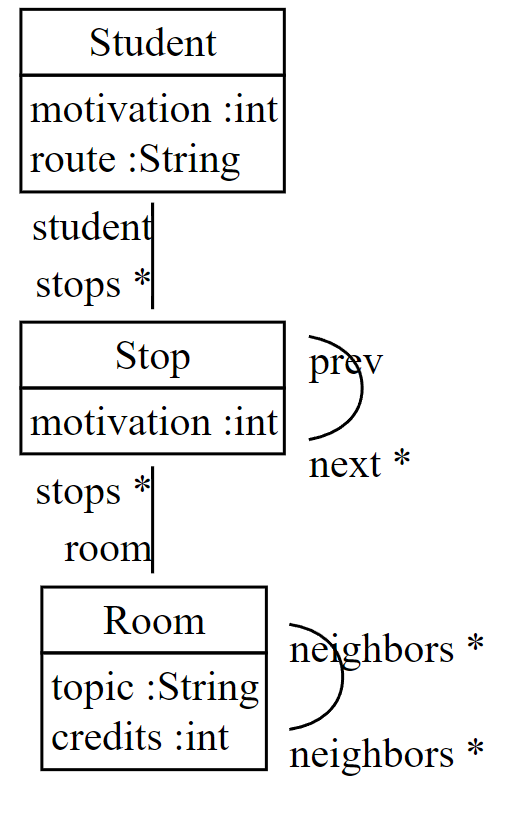
\includegraphics[width=0.25\textwidth]{images/3.1.4/class_diagram}
    \caption{Mittels fulibWorkflows generiertes Klassendiagramm}
    \label{fig:generated-class}
\end{figure}

In Abbildung~\ref{fig:generated-class} ist das im vorherigen Kapitel verwendete Beispiel zur Grundlage der Generierung eines Klassendiagramms genutzt worden.
Das Klassendiagramm besteht aus drei Klassen und beinhaltet alle beschriebenen Assoziationen bestehend aus Kanten, Bezeichnern an beiden Seiten und den entsprechenden
Kardinalitäten.
Bei den Kardinalitäten kennzeichnet ein ``*'' eine To-Many-Assoziation.
Die Typen der Felder einer Klasse können lediglich zwischen ``String'' und ``int'' unterschieden werden.
